\documentclass[11pt]{beamer}
\usetheme{Warsaw}

\usepackage[utf8]{inputenc}
\usepackage[russian]{babel}
\usepackage[T2A]{fontenc}
\usepackage{amsmath}
\usepackage{amsfonts}
\usepackage{amssymb}
\usepackage{graphicx}

\usepackage[most]{tcolorbox}

%\usepackage{appendixnumberbeamer}
 
\newtheorem{rustheorem}{Теорема }
\DeclareMathOperator*{\argmin}{argmin}
\let\T\intercal
\let\ov\overline
\def\bar_#1{\bold{\ov{#1}}}
\def\hatup_#1{\bold{\hat{#1}}}
\def\ton_#1{1,2,\dots,#1}
\def\msf_#1{\mathsf{#1}}
\def\Lagr{\mathcal{L}}
\def\bo_#1{\bold{#1}}
\def\trans{^\intercal}

\setbeamersize{text margin left=10pt,text margin right=10pt} 

\setbeamertemplate{footline}
{
  \leavevmode%
  \hbox{%
  \begin{beamercolorbox}[wd=.25\paperwidth,ht=2.25ex,dp=1ex,center]{author in head/foot}%
    \usebeamerfont{author in head/foot}\insertshortauthor
  \end{beamercolorbox}%
  \begin{beamercolorbox}[wd=.75\paperwidth,ht=2.25ex,dp=1ex,center]{title in head/foot}%
    \usebeamerfont{title in head/foot}\insertshorttitle\hspace*{3em}
  \end{beamercolorbox}}%
  \vskip0pt%
}

%
\makeatletter
\setbeamertemplate{headline}
{%
  \leavevmode%
  \@tempdimb=2.4375ex%
  \ifnum\beamer@subsectionmax<\beamer@sectionmax%
    \multiply\@tempdimb by\beamer@sectionmax%
  \else%
    \multiply\@tempdimb by\beamer@subsectionmax%
  \fi%
  \ifdim\@tempdimb>0pt%
    \advance\@tempdimb by 1.825ex%
    \begin{beamercolorbox}[wd=.25\paperwidth,ht=\@tempdimb]{section in head/foot}%
      \vbox to\@tempdimb{\vfil\insertsectionnavigation{.25\paperwidth}\vfil}%
    \end{beamercolorbox}%
    \begin{beamercolorbox}[wd=.75\paperwidth,ht=\@tempdimb]{subsection in head/foot}%
      \vbox to\@tempdimb{\vfil\insertsubsectionnavigation{.75\paperwidth}\vfil}%
    \end{beamercolorbox}%
  \fi%
}

\author{Андрей Квасов}
\title{Отчет по преддипломной практике}
\subtitle{Реализация процедуры оценивания динамичеcкой структуры инвестиционного портфеля хедж-фонда}
%\setbeamercovered{transparent} 
\setbeamertemplate{navigation symbols}{} 
%\logo{} 
\institute{МГУ им. М.\ В.\ Ломоносова} 
\date{12 февраля 2016} 
%\subject{}

\begin{document}

\begin{frame}
\maketitle
\end{frame}

%\begin{frame}
%\tableofcontents
%\end{frame}


\section{Обзор предметной области и постановка задачи}
\begin{frame}{Задача распознавания сигналов}
\begin{itemize}
\item Объектом распознавания являются сигналы $\bo_x = (\bo_x_1,\dots,\bo_x_N), \bo_x_i \in \mathbb{R}^n, i=1,\dots,N$. Целевая переменная - $\bo_y \in \mathbb{R}^N$.
\item Рассматривается модель нестационарной линейной регрессии, где искомой величиной является сигнал $\bo_{\beta} = (\bo_{\beta}_1,\dots,\bo_\beta_N)$, связанный с целевым вектором $\bo_y_t = \bo_x_t^\T\bo_\beta_t + \varepsilon_t$. 
\item Модель динамики изменения сигнала $\bo_{\beta}_t = V_t\bo_{\beta}_{t-1} + \varepsilon^\prime_t$
\end{itemize}
\end{frame}

\begin{frame}{Обзор предметной области}
\framesubtitle{Style analysis инвестиционного портфеля}
\begin{columns}[T]
    \begin{column}{.5\textwidth}
     \begin{block}{Returns Based Style Analysis model}
		$z_t^i$ - цена актива в портфеле\\
		$m_t^i$ - количество активов в портфеле, данного вида\\
		$x_t^i = \frac{z_t^i - z_{t-1}^i}{z_{t-1}^i}$ - доходности активов в портфеле\\
    \end{block}
    \end{column}
    \begin{column}{.5\textwidth}
   	 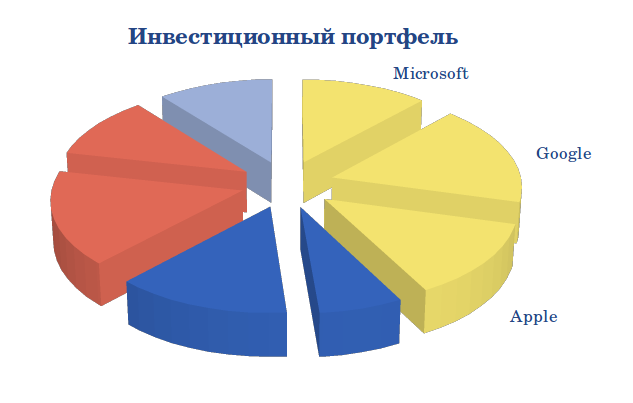
\includegraphics[width=\textwidth]{pic1.png}
    \end{column}
  \end{columns}
\end{frame}
	
\begin{frame}{Обзор предметной области}
\framesubtitle{Style analysis инвестиционного портфеля}
\begin{columns}[T]
    \begin{column}{.5\textwidth}
     \begin{block}{Returns Based Style Analysis model}
		$\hat{y}_t = \sum_{i=1}^n m_t^iz_t^i$ - стоимость инвестиционного портфеля (скрытая величина)\\
		$y_t = \frac{\hat{y}_t - \hat{y}_{t-1}}{\hat{y}_{t-1}}$ - доходность портфеля (наблюдаемая величина)\\
		$\hat{\beta}_t^i = \frac{m_t^i z_t^i}{\sum_{i=1}^n m_t^i z_t^i}$ - доля актива $i$ в портфеле\\
		$x_t^0$ --- доходность безрискового актива ($x_t^0 \approx x^0\ \forall t=1,\dots,N$)\\
    \end{block}
    \end{column}
    \begin{column}{.5\textwidth}
   	 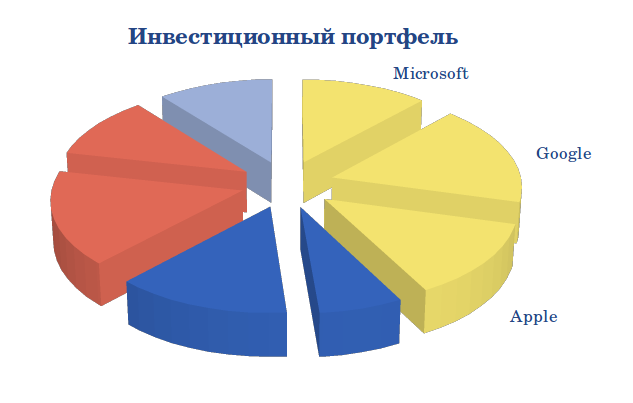
\includegraphics[width=\textwidth]{pic1.png}\\
   	\qquad\qquad \[
\begin{cases}
y_t = \bo_x_t^\T \bo_\beta_t + \varepsilon_t^1, \text{ где } \bo_\beta_t \approx \bo_{\hat{\beta}}_t \\
\sum_{i=1}^n \beta_t^i = 1
\end{cases}
\]
    \end{column}
  \end{columns}
\end{frame}


\begin{frame}{Постановка задачи}
\framesubtitle{Модели нестационарной регрессии и динамики изменения сигнала}
\begin{block}{Модель наблюдения, нестационарно регрессии: узловые функции }
\[
\sum\limits_{t = 1}^N {q({y_t},{{\bf{x}}_t},{{\bf{\beta}}_t})}  = \sum\limits_{t = 1}^N {{{({y_t} - {\bf{\beta}}_t^T{{\bf{x}}_t})}^2}}
\]
\end{block}

\begin{tcolorbox}[beamer,title=Модель динамики: функции связи,height=3cm, colback=blue!5!white,colframe=blue!50!black]
$
\sum\limits_{t = 2}^N \nu({\bf{\beta}}_t, {\bf{\beta}}_{t-1}| \lambda) = \sum\limits_{t = 2}^N {{({{\bf{\beta}}_t} - \,{{\bf{V}}_t}{{\bf{\beta}}_{t - 1}})}\trans}{\bf{U}}_t({{\bf{\beta}}_t} - \,{{\bf{V}}_t}{{\bf{\beta}}_{t - 1}})$\\
$\msf_U_t = \msf_{Diagonal}(\lambda)$, где $\lambda$ --- параметр сглаживания $V_t$ --- матрица динамики сигнала, $V_t = E$ --- едничная
\end{tcolorbox}
\end{frame}

\begin{frame}{Постановка задачи}
\framesubtitle{Полный критерий обучения}
\begin{tcolorbox}[beamer,title=Общий критерий для оценивания состава портфеля,height=2.3cm, colback=blue!5!white,colframe=blue!50!black]
\[
J({\bf{\beta}}_1,\dots, {\bf{\beta}}_N|\lambda) = \sum\limits_{t = 1}^N q({y_t},{{\bf{x}}_t},{{\bf{\beta}}_t}) + \sum\limits_{t = 2}^N \nu({\bf{\beta}}_t, {\bf{\beta}}_{t-1}| \lambda)
\]
\end{tcolorbox}
\begin{block}{Задача программирования с парно-сепарабельной функцией}
\[\begin{cases}
\msf_J(\bold \beta_1, \dots, \bold \beta_N|\lambda)\to \min \left( {({{\bf{\beta}}_1},\dots,{{\bf{\beta}}_N})\, \in \,{\mathbb R^{n\times N}}} \right)\\
\sum_{i=1}^n \beta_t^i = 1,\ t=1,\dots,N
\end{cases}
\]
\end{block}
\begin{block}{Постановка задачи преддипломной практики}
Исследование методов подбора структурного параметра $\lambda$ для модели нестационарной регрессии в задаче восстановления скрытой стратегии управления инвестиионным портфелем.
\end{block}
\end{frame}

\section{Математическое исследование задачи}
\begin{frame}{Динамические методы обучения}
\framesubtitle{Метод прогонки}
\begin{block}{Учет ограничений равенств}
$\beta_t^0 = 1-\sum_{i=1}^n \beta_t^i$ приходим к выражению $y_t-x_t^0 = \sum_{i=1}^n(x_t^i-x_t^0)\beta_t^i$, т.о. $\tilde{y}_t^i = \sum_{i=1}^n\tilde{x}_t^i\beta_t^i$. Переобозначим обратно.
\end{block}
Дифференцирование по аргументам критерия  $({{\bf{\beta}}_1},\dots,{{\bf{\beta}}_N})$, тогда получим реккурентное соотношение для каждого вектора $t=1,\dots,N$: $A_t {{\bf{\beta}}_{t-1}} + B_t {{\bf{\beta}}_t} + C_t{{\bf{\beta}}_{t+1}} = F_t$, где 
\begin{align*} &A_t = -U_t V_t;\ B_t = \begin{cases}(x_t x_t \trans + U_{t+1}\trans U_{t+1}V_{t+1}),\ t=1\\ (x_t x_t \trans + U_t + U_{t+1}\trans U_{t+1}V_{t+1}),\ t=2,\dots,N-1\\ (x_t x_t \trans + U_t),\ t=N\end{cases};\\ &C_t =-V_{t+1}\trans U_{t+1}; A_t \in \mathbb R^{n\times n},\ B_t \in \mathbb R^{n\times n},\ C_t \in \mathbb R^{n\times n}
\end{align*}
\end{frame}

\begin{frame}{Динамические методы обучения}
\framesubtitle{Метод прогонки}
\begin{equation*}
    \label{matrix_progonka}
    Q = \begin{pmatrix}
    B_1   & C_1 & 0 & \dots  & \dots     & \dots     & \dots     & 0         \\
    A_2   & B_2                      & C_2                   & \dots  & \dots     & \dots     & \dots     & 0         \\
    0      & A_3                      & B_3                   & C_3   & \dots     & \dots     & \dots     & 0         \\
    \vdots & \vdots                    & \ddots                 & \ddots & \ddots    &           &           & \vdots    \\
    \vdots &                           & \ddots                 & \ddots & \ddots    & \ddots    &           & \vdots    \\
    \vdots &                           &                        & \ddots & A_{N-2} & B_{N-2} & C_{N-2} & 0         \\
    0      & \dots                     & \dots                  & \dots  & 0         & A_{N-1} & B_{N-1} & C_{N-1} \\
    0      & \dots                     & \dots                  & \dots  & 0         & 0         & A_N      & B_N     
    \end{pmatrix}
\end{equation*}
Тогда считая ${\bf \hat \beta} = (\beta_t^i,\ i=1,\dots,n,\  t=1,\dots,N) \in \mathbb R^{nN}$ и ${\bf \hat x} = (x_t^i,\ i=1,\dots,n,\  t=1,\dots,N) \in \mathbb R^{nN}$: Ищем решение системы
$Q {\bf \hat \beta} = {\bf \hat x}$
\end{frame}

\begin{frame}{Динамические методы обучения}
\framesubtitle{Метод Беллмана}
\begin{columns}[T]
\begin{column}{.5\textwidth}
   	  \begin{block}{Левые функции Беллмана}
Частичный критерий:\ 
		$\msf_J_t^{-}(\bar_\beta_1, \dots, \bar_\beta_t) = \sum_{i=1}^t \psi_i(\bar_\beta_i) + \sum_{i=2}^t \gamma_i(\bar_\beta_{i-1}, \bar_\beta_i)$\\
Функция Беллмана:\\
		$\tilde{\msf_J}_t^{-}(\bar_\beta_t) = \displaystyle\min_{\bar_\beta_1,\dots,\bar_\beta_{t-1}}\msf_J_t^{-}(\bar_\beta_1, \dots, \bar_\beta_t) $\\
Рекуррентное соотношение:\
		$\tilde{\msf_J}_t^{-}(\bar_\beta_t) =\psi_t(\bar_\beta_t) +  \displaystyle\min_{\bar_\beta_{t-1}}[\gamma_t(\bar_\beta_{t-1}, \bar_\beta_t)+\tilde{\msf_J}_{t-1}^{-}(\bar_\beta_{t-1})]$\\
    \end{block}
    \end{column}
    \begin{column}{.5\textwidth}
     \begin{block}{Правые функции Беллмана}
Частичный критерий:\ 
		$\msf_J_t^{+}(\bar_\beta_t, \dots, \bar_\beta_N) = \sum_{i=t}^N \psi_i(\bar_\beta_i) + \sum_{i=t+1}^N \gamma_i(\bar_\beta_{i-1}, \bar_\beta_i)$ \\
Функция Беллмана:\
		$\tilde{\msf_J}_t^{+}(\bar_\beta_t) = \displaystyle\min_{\bar_\beta_{t+1},\dots,\bar_\beta_N}\msf_J_t^{+}(\bar_\beta_t, \dots, \bar_\beta_N)$\\
Рекуррентное соотношение:\
		$\tilde{\msf_J}_t^{+}(\bar_\beta_t) =\psi_t(\bar_\beta_t) + \displaystyle\min_{\bar_\beta_{t+1}}[\gamma_{t+1}(\bar_\beta_{t}, \bar_\beta_{t+1})+\tilde{\msf_J}_{t+1}^{-}(\bar_\beta_{t+1})]$\\
    \end{block}
    \end{column}
\end{columns}
\qquad Искомые значения $\bar_\beta_t = \displaystyle\min_{\bar_\beta_t}[\tilde{\msf_J}_t^{-}(\bar_\beta_t) + \tilde{\msf_J}_t^{+}(\bar_\beta_t) - \psi(\bar_\beta_t)]$
\end{frame}

\begin{frame}{Оценки структурного параметра $\lambda$}
\framesubtitle{Оценки по кросс-валидации, Predicted R2} %[r]
\begin{block}{Leave One Out}
\[
LOO = \frac1{N^2} \sum_{k=1}^N \sum_{t=1}^N (y_t - \sum_{i=1}^n \tilde{\beta}_t^{i^k} x_t^i)^2
\], где $\tilde{\beta}_t^{i^k}$ - обученные доли активов для контрольного объекта ${\bf{x}}_t$.
\end{block}
\begin{block}{Leave Half Out}
\[
LHO = \frac12 \sum_{t=1}^N \left( (y_t - \sum_{i=1}^n (\tilde{\beta}_t^i){}^{\prime} x_t^i)^2 + (y_t - \sum_{i=1}^n (\tilde{\beta}_t^i){}^{\prime\prime} x_t^i)^2 \right)
\], где $(\tilde{\beta}_t^i){}^{\prime}$ - доли активов, в обучении участвуют объекты с нечетным индексом , а $(\tilde{\beta}_t^i){}^{\prime\prime}$ - доли ... c четным индексом $t$
\end{block}
\end{frame}

\begin{frame}{Оценки структурного параметра $\lambda$}
\framesubtitle{Модификация информационного критерия Акаике, общий случай (AIC)} %[r]
\begin{block}{AIC}
\begin{align*}
    \hat \lambda ({\bf{y}},{\bf{X}})\, &= \,\mathop {\arg \min }\limits_\lambda  \left\{ {\frac{1}{{2{\sigma ^2}}}} \right.{{\left( {{\bf{y}}\, - \,{{\bf{X}}^T}{{{\bf{\hat \beta}}}_\lambda }({\bf{y}},{\bf{X}})} \right)}^T}\left( {{\bf{y}}\, - \,{{\bf{X}}^T}{{{\bf{\hat \beta}}}_\lambda }({\bf{y}},{\bf{X}})} \right) \\&+ \Delta (\lambda ,{\bf{X}})\left.  \right\}, \text{где} \Delta (\lambda ,{\bf{X}}) = Tr\left[ {{\bf{X}}{{\bf{X}}^T}{{\left( Q \right)}^{-1}}} \right]
\end{align*}
\end{block}
${\bf{X}}$ составлена из векторов $x_t$ стоящих своими элменетами в виде столбца в $t*n$ столбике матрицы ${\bf{X}}$, по строкам  позициях с $t*n$ по $({t+1})*n$. $\sigma^2$ - дисперсия нормального распределения $\Phi(y_t| \bf{x}_t)$.\\ 
\cite{aic_modif} \emph{Обобщение информационного критерия Акаике для выбора значений непрерывного параметра в моделях данных} / В. В. Моттль, О. В. Красоткина, Е. О. Ежова (Черноусова)
\end{frame}

\section{Вычислительные эксперименты}
\begin{frame}{Исходные данные}
\begin{itemize}
\item Данные предоставленные компанией "Markov Processe Int.": Доходности (в процентах) для 158 фондов, 12 активов, 120 дней (конец 2014, первый квартал 2015 года)
\item Используются 60 дней, все 12 активов (включая и безрисковый)
\item Эксперименты проводятся с каждым фондом отдельно, для исследования в отчете используется первый фонд  "Wells Fargo Funds Trust: Wells Fargo Advantage Opportunity Fund; Investor Class Shares".
\item Для поиска оптимума $\lambda$ выбиралась сетка с 13 значениями от 1 до 800 в логарифмической шкале (по основанию 2) 
\end{itemize}
\end{frame}

\begin{frame}{Исходные данные}

\begin{figure}
\centering
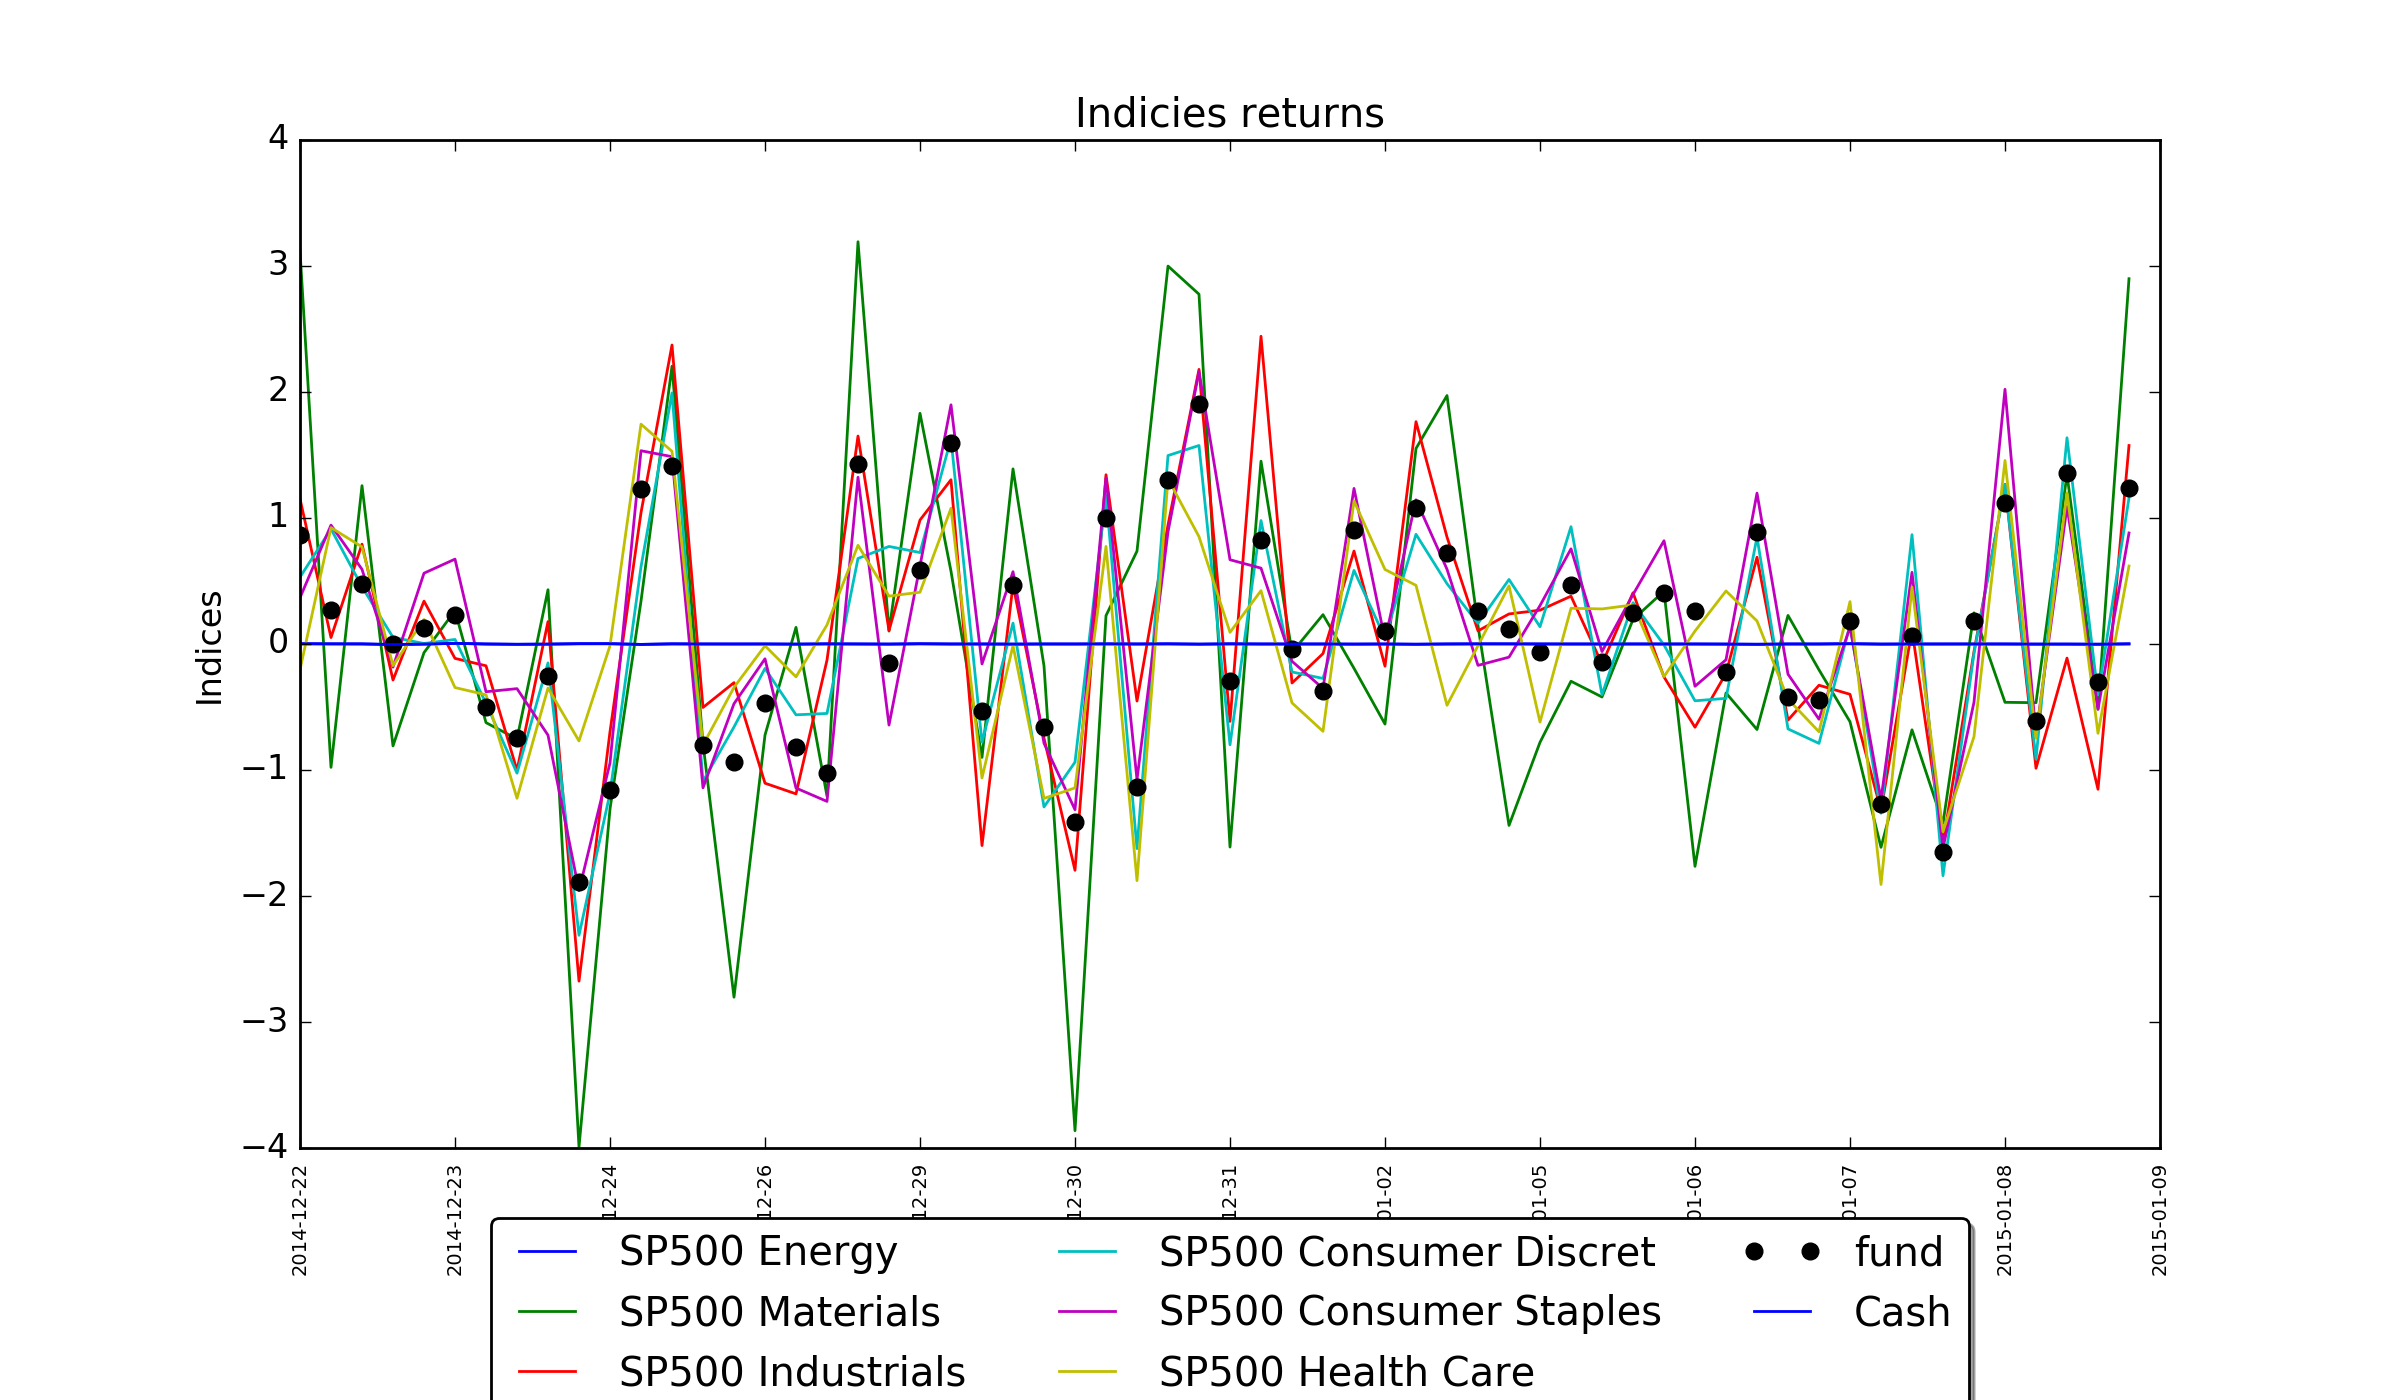
\includegraphics[width=0.8\textwidth]{assets.png}
\caption{Индекс SP500 в разных сферах (первые 6 признаков), доходность портфеля фонда (черные кружки)}
\ref{fig:assets}
\end{figure}

\end{frame}


\begin{frame}{Применение модели нестационарной регрессии}
\framesubtitle{Пример применения модели с $\lambda = 1$}

\begin{figure}
\centering
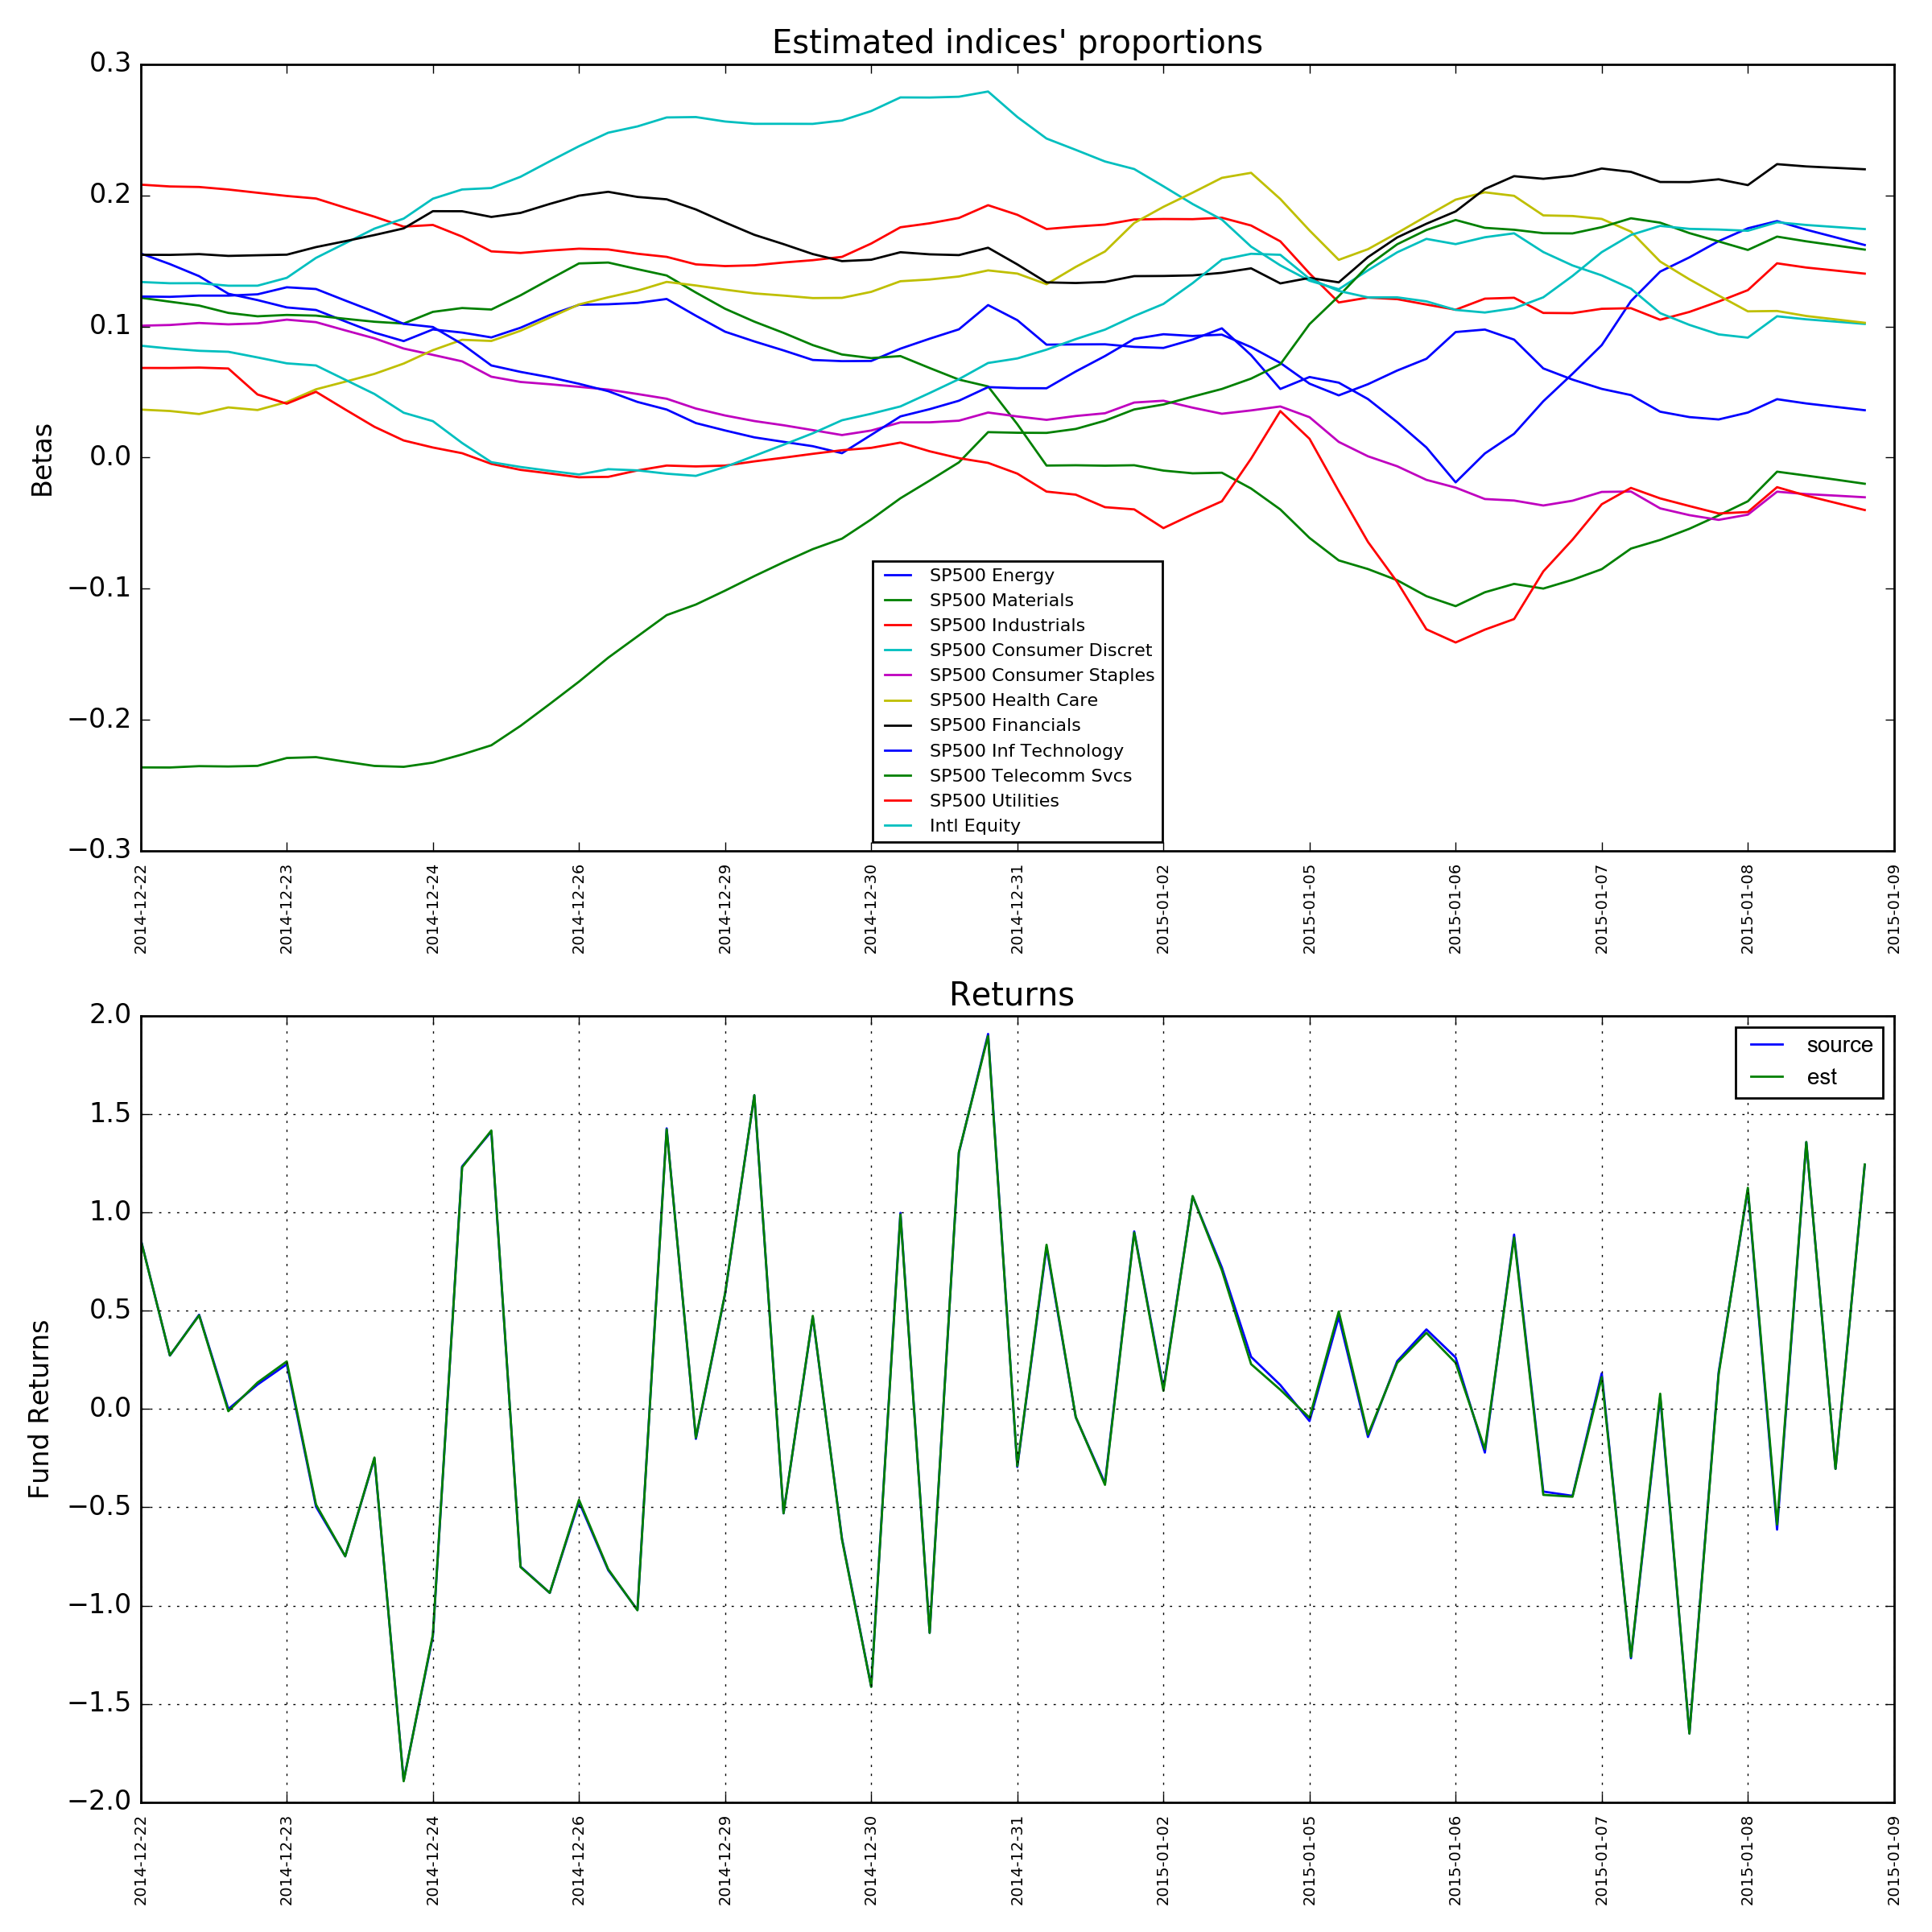
\includegraphics[scale=0.2]{example_nsr.png}
\end{figure}

\end{frame}

\begin{frame}{Применение модели нестационарной регрессии}
\framesubtitle{Leave One Out и проблема коррелированных признаков}

\begin{figure}
\centering
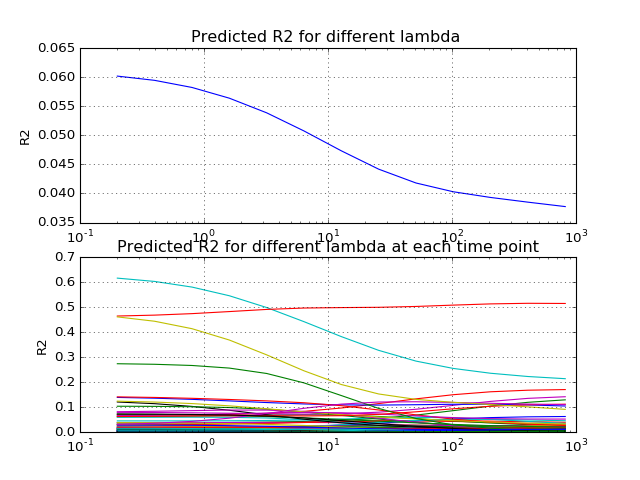
\includegraphics[scale=0.4]{loo_r2.png}
\end{figure}
\end{frame}

\begin{frame}{Применение модели нестационарной регрессии}
\framesubtitle{Leave One Out и проблема коррелированных признаков}

\begin{figure}
\centering
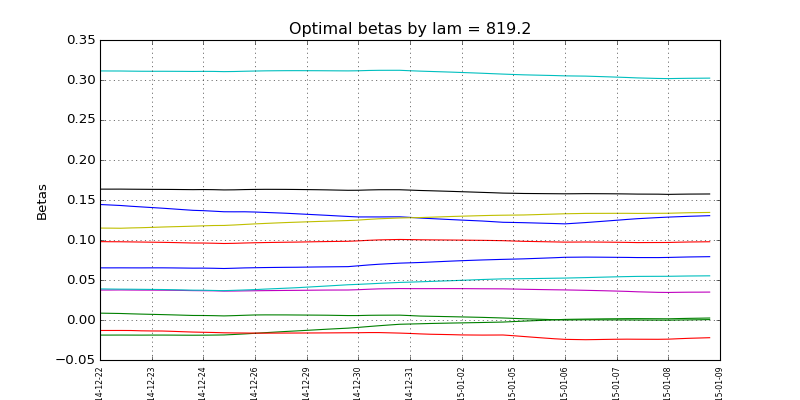
\includegraphics[scale=0.25]{loo_beta.png}\\
\centering
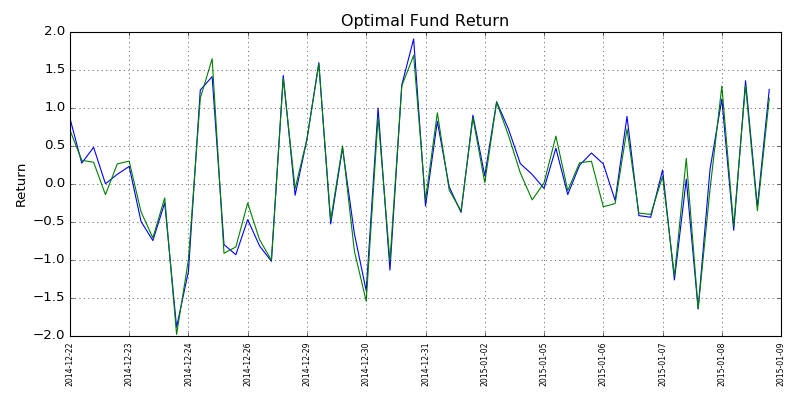
\includegraphics[scale=0.25]{loo_return.png}
\end{figure}
\end{frame}

\begin{frame}{Применение модели нестационарной регрессии}
\framesubtitle{Проблема коррелированных признаков, переход к пространству скрытых факторов}
\begin{itemize}
\item Рассмотрим собственные вектора ${\bf{z}}_i,\ i=1,\dots,N$ матрицы ${\bf{M}} \in \mathbb R^{N\times N}$ корреляции данных ${\bf{X}} = ({\bf{x}}_1,\dots, {\bf{x}}_N) \in \mathbb R^{N\times N}: {\bf{M}}_{ij} = {\bf{x}}_i {\bf{x}}
_j\trans $
\item Все кроме первых $n=11$ наибольших собственных значений близки к нулю, тогда берем первые $m \leq n$ векторов ${\bf{z}}_i$, так что ${\bf{Z}} = ({\bf{z}}_1, \dots, {\bf{z}}_m)$ - выборка скрытых факторов, которые выражают любой наш исходный сигнал с помощью матрицы ${\bf{A}}: {\bf{x}}_t = {\bf{A}} {\bf{z}}_t,\ t=1,\dots, N$. 
\item ${\bf{A}}$ --- матрица с собственными векторами матрицы ${\bf{M}}^\prime = \sum_{t=1}^N x_t\trans x_t $ в виде столбцов.
\end{itemize}

\end{frame}

\begin{frame}{Применение модели нестационарной регрессии}
\framesubtitle{Переход к пространству скрытых факторов}
\begin{figure}
\centering
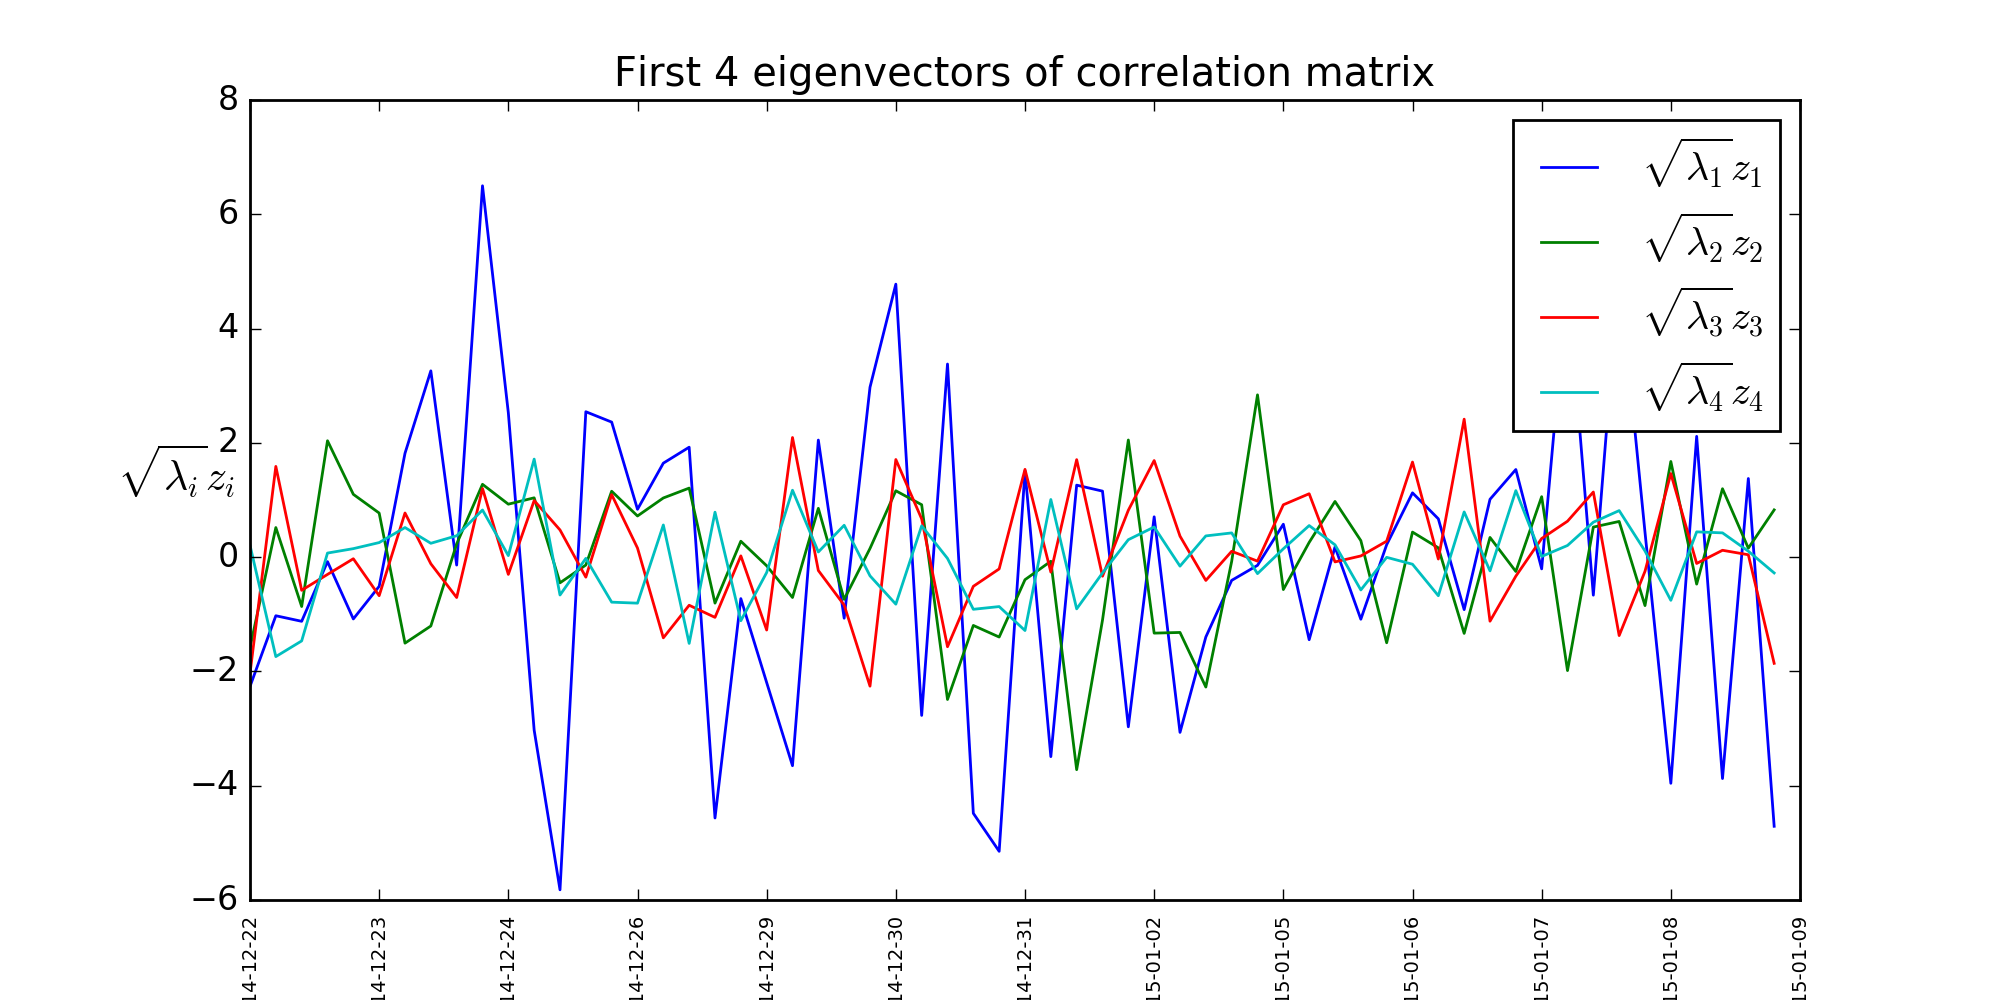
\includegraphics[scale=0.5]{eigvecs.png}\\
\end{figure}
\end{frame}


\begin{frame}{Применение модели нестационарной регрессии}
\framesubtitle{Leave One Out в пространстве скрытых факторов}
\begin{figure}
\centering
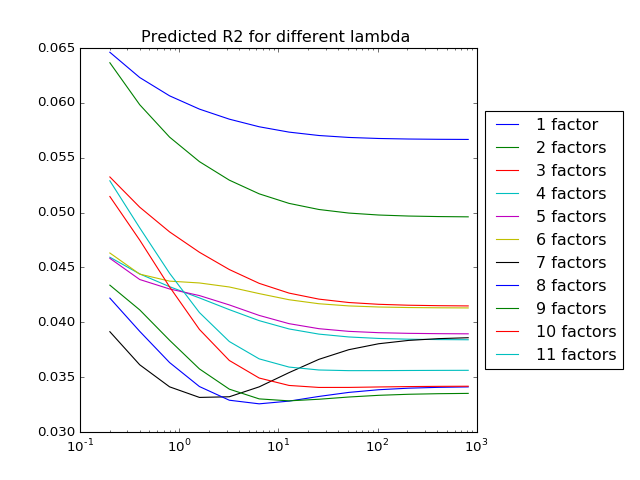
\includegraphics[scale=0.4]{looeig_r2.png}
\end{figure}
\end{frame}

\begin{frame}{Применение модели нестационарной регрессии}
\framesubtitle{Leave One Out в пространстве скрытых факторов}
\begin{figure}
	\centering
	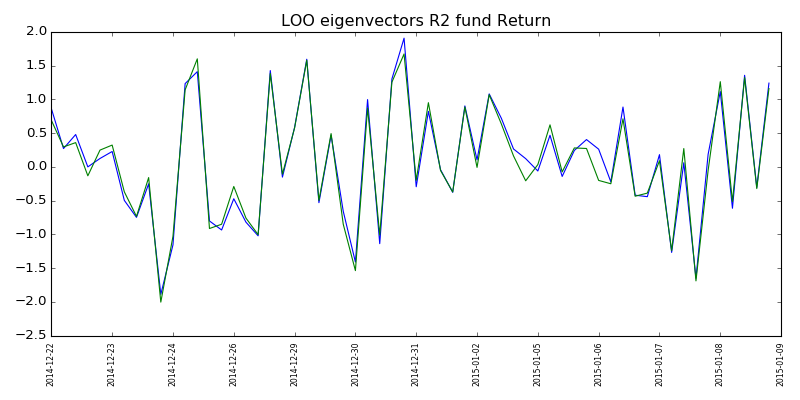
\includegraphics[scale=0.38]{looeig_return.png}
	\caption{Доходность портфеля при выборе оптимума $m=8,\lambda=6.4$ методом LOO\_eigen}
\end{figure}
\end{frame}

\begin{frame}{Применение модели нестационарной регрессии}
\framesubtitle{Leave Half Out}

\begin{figure}
\centering
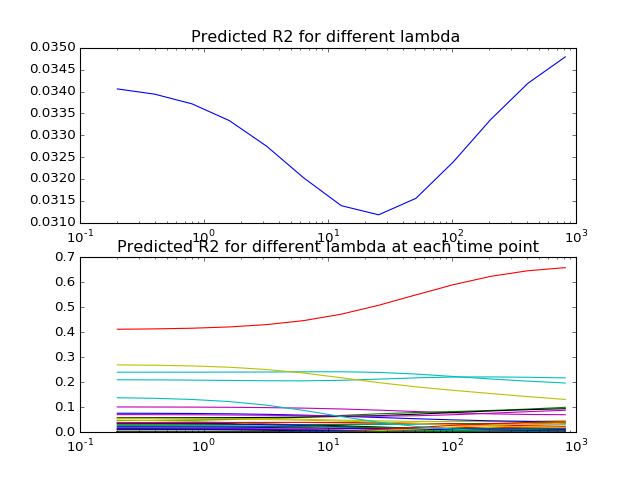
\includegraphics[scale=0.4]{lho_r2.png}
\end{figure}
\end{frame}

\begin{frame}{Применение модели нестационарной регрессии}
\framesubtitle{Leave Half Out}

\begin{figure}
\centering
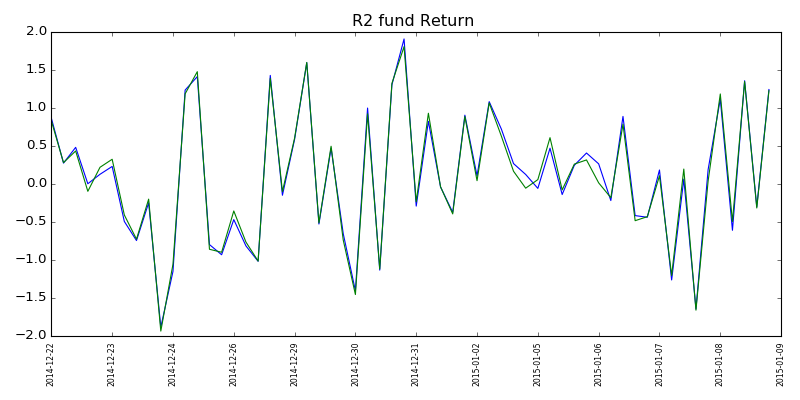
\includegraphics[scale=0.38]{lho_return.png}
\caption{Доходность портфеля при выборе оптимума $\lambda=25.6$}
\end{figure}
\end{frame}

\begin{frame}{Применение модели нестационарной регрессии}
\framesubtitle{AIC}
\begin{figure}
\centering
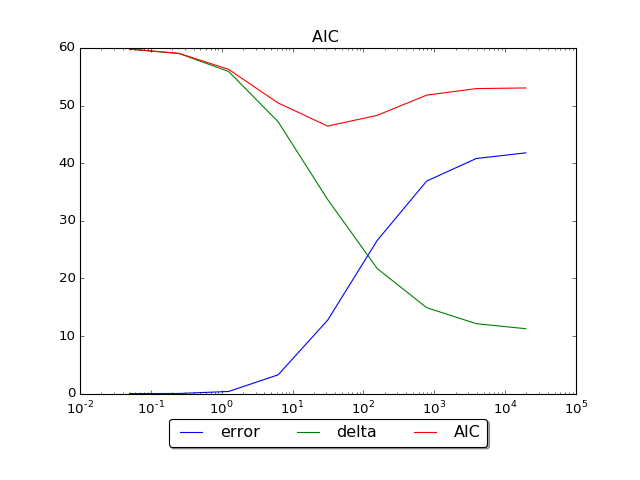
\includegraphics[scale=0.4]{aic_r2.png}
\end{figure}
\end{frame}

\begin{frame}{Применение модели нестационарной регрессии}
\framesubtitle{AIC}
\begin{figure}
\centering
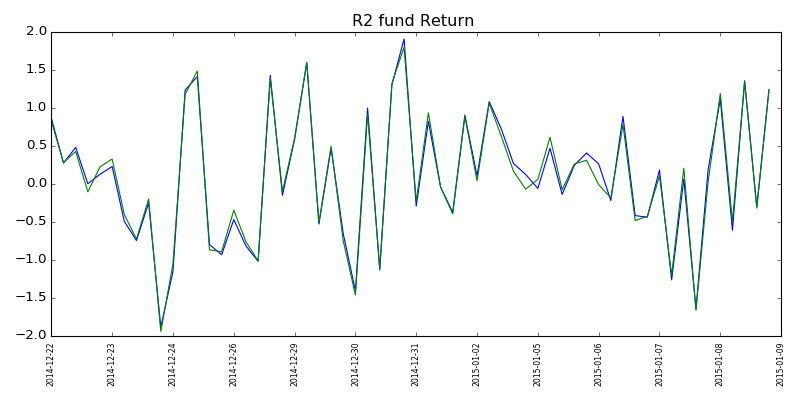
\includegraphics[scale=0.4]{aic_return.png}
\caption{Доходность портфеля при выборе оптимума $\lambda=31.25$}
\end{figure}
\end{frame}

\section{Выводы}
\begin{frame}{Применение модели нестационарной регрессии}
\framesubtitle{Return Based Style Analysis}
\begin{figure}
\centering
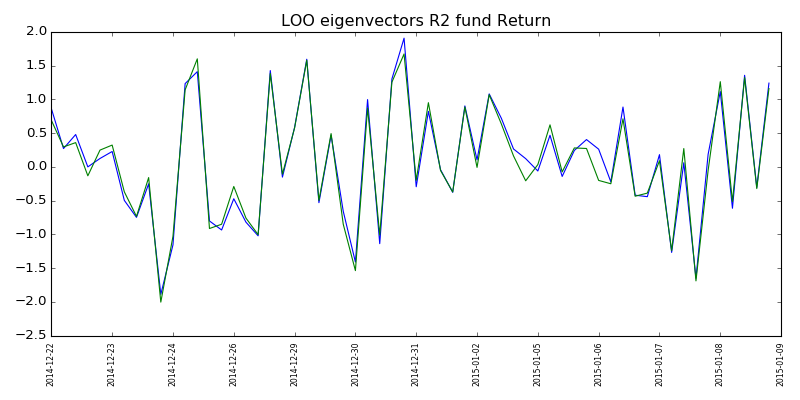
\includegraphics[scale=0.22]{looeig_return.png}
\centering
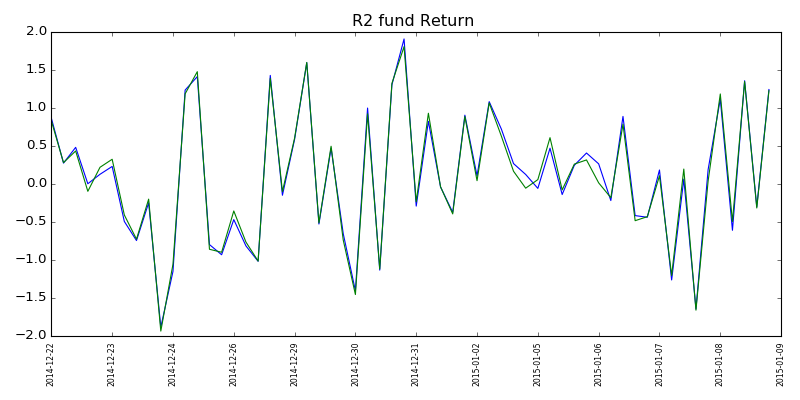
\includegraphics[scale=0.22]{lho_return.png}\\
\centering
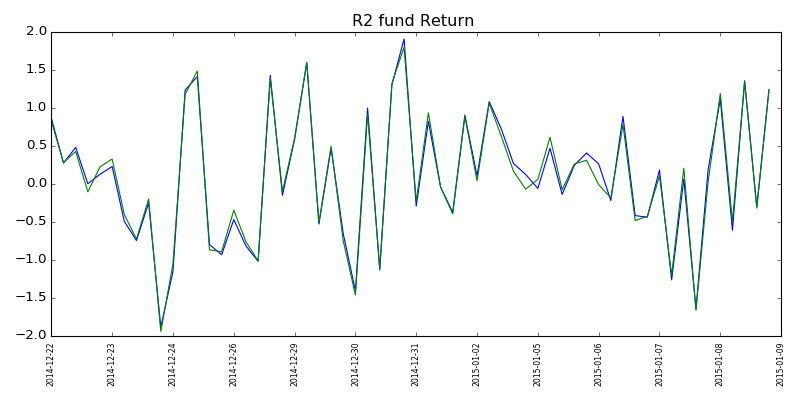
\includegraphics[scale=0.22]{aic_return.png}
\end{figure}
\end{frame}

\section{Заключение}
\begin{frame}
\begin{itemize}
\item Реализованы программные средства для решения задачи восстановления  скрытого управления инвестиционным портфелем
\item Реализованы методы оценивания структурного параметра $\lambda$, проведен анализ применимости методов к реальным данным инвестиционных портфелей.
\item Произведена подготовительная исследовательская работа на тему ВКР "Использование критерия обоснованности модели для подбора структурных элементов в задаче восстановления скрытой стратегии управления инвестиционным портфелем".
\end{itemize}
\end{frame}

%\begin{frame}
%\end{frame}

\begin{thebibliography}{100} % 100 is a random guess of the total number of references
\section{Литература}

\begin{frame}
\bibitem{bellman} Bellman R. Dynamic Programming. Princeton University Press, Princeton, N.J., 1957.
\bibitem{dynamic} Алгоритмы Динамического Программирования для Анализа Нестационарны сигналов / В.В. Моттль, А.А. Костин, О.В. Красоткина
\bibitem{theory} Беспереборная кросс-валидация отбора признаков в линейной регрессионной модели / О. В. Красоткина, В. В. Моттль, Н. А. Разин, Е. О. Черноусова // Известия ТулГУ. Технические науки. – 2013. – Вып. 7. – No. 2. – С. 88-98.
\end{frame}

\begin{frame}
\bibitem{aic_orig} Akaike, H. Information theory and an extension of the maximum likelihood principle. // Proc. 2nd Intern. Symp. Inf. Theory, Petrov P.N. and Csaki F. eds. Budapest. – 1973. – P. 267-281. 
\bibitem{aic_modif} Обобщение информационного критерия Акаике для выбора значений непрерывного параметра в моделях данных / В. В. Моттль, О. В. Красоткина, Е. О. Ежова (Черноусова) // Труды 51 научной конференции МФТИ «Современные проблемы фундаментальных и прикладных наук». — 2008. — Т. 3. — С. 58-60.
\end{frame}


\end{thebibliography}

\end{document}
